\documentclass[12pt,a4paper]{article}
\usepackage[top=1in, bottom=1in, left=1.25in, right=1.25in]{geometry} 
\usepackage{url}
\usepackage{fancyhdr}
\usepackage[UTF8]{ctex}
\usepackage{listings}
%\usepackage[hyphens]{url}
\usepackage{setspace}
\usepackage{enumitem}
\usepackage{float}
\usepackage{ltablex}
\usepackage{booktabs}
\usepackage{float}
\usepackage{tabu}
\usepackage{indentfirst}
\usepackage{booktabs}
\usepackage{amsmath}
\usepackage{graphicx}
\usepackage{tikz}
\usepackage[final]{pdfpages}
\usepackage[linesnumbered,lined,ruled,vlined,commentsnumbered]{algorithm2e}


\fancyhf{}
\lhead{信息可视化}
\rhead{伪基站数据可视化}
\cfoot{\thepage}

\usetikzlibrary{shapes}

\setlength{\parindent}{2em}
\setlist[enumerate]{
	listparindent=\parindent
}

\setkeys{Gin}{keepaspectratio, width=0.8 \textwidth}

\pagestyle{fancy}

\begin{document}
\thispagestyle{plain}
\begin{center}
	{\LARGE \textbf{浙江大学实验报告} \par}
\end{center}
\begin{flushleft}
课程名称:\uline{信息可视化} \hfill 实验项目名称:\uline{伪基站数据可视化} \hfill 实验类型:\uline{综合型} \\

学生姓名:\uline{汪砚戎} \hfill  专业:\uline{计算机科学与技术} \hfill 学号:\uline{3150104945}

学生姓名:\uline{郝广博} \hfill  专业:\uline{计算机科学与技术} \hfill 学号:\uline{3150104785}

学生姓名:\uline{周晟皓} \hfill  专业:\uline{计算机科学与技术} \hfill 学号:\uline{3150103078}

\end{flushleft}

\section{设计需求}

在当下移动终端设备使用越来越为广泛的年代,垃圾短信对人们的日常生活可以说是影响越来越大。
而我们所常说的“伪基站”即假基站,其能够搜集以其为中心、一定半径范围内的手机卡信息,并利用GSM验证漏洞来伪装成运营商的基站来
发送垃圾短信。
相较于其他种类的垃圾短信,由伪基站所发送的垃圾短信由于其能够模拟各种不同的号码来发送垃圾短信,因而其若是
冒用银行、运营商等机构的号码来发送垃圾短信甚至是诈骗短信之时,其危害性可以说是相当大的。除此之外,由于伪基站发送垃圾短信的成本
极低,因而其的垃圾短信的发送量可以说是相当大的,因而其不仅常常会干扰公共的无线频率资源,有时候甚至可能会影响人们的正常通讯。
除此之外,有些伪基站所发送的短信中还附带了恶意病毒和木马的下载链接,用户若是不小心下载之后便可能造成手机中毒、个人信息被盗、
资金被盗刷等恶劣影响。除此之外,部分不法人员还通过伪基站大量群发内容不受控的短信息,可以说是严重地侵害了社会秩序。
因而对我们来说,我们必须要大力打击不法的伪基站。

而现在,QHNet公司公开了一部分由其手机卫士应用软件所收集到的垃圾短信的数据。
该数据集的内容十分丰富,其包含了大约300多万条在北京地区被用户标注的垃圾短信样本数据,其中每一条短信都包含
正文、接收时间、发送者号码以及接收该条垃圾短信前最后连接的正常合法基站信息。
然而,伪基站有非常强的流动性,因此依据近似位置和传统数据分析方法,仍然很难准确把握伪基站的活动规律。
而如果我们能够充分利用此一数据集并对其通过运用可视化的方法来揭示伪基站的行为模式,就一定可以为有关部门打击伪基站
做出极大的贡献,从而对保卫普通人民群众的财产安全,维护我国清朗的网络环境尽上一份力。

\section{设计介绍}

在我们的设计中,我们主要是运用数据可视化的方法来揭示伪基站的活动规律。
我们可视化的主要方法是将北京地区的地图分为许多个大小相同的小方格,并根据我们收集到的数据里该方格内的垃圾短信的数量来给该方格
上色,从而可以让我们对北京地区垃圾短信的分布有一个直观上的了解。除此之外,我们还可以利用将鼠标移动到每个小方格上的方法,查看
该方格内各类垃圾短信的具体数量,从而得以了解各类垃圾短信的主要类型。



\begin{flushleft}
\begin{figure}[H]
	\centering
		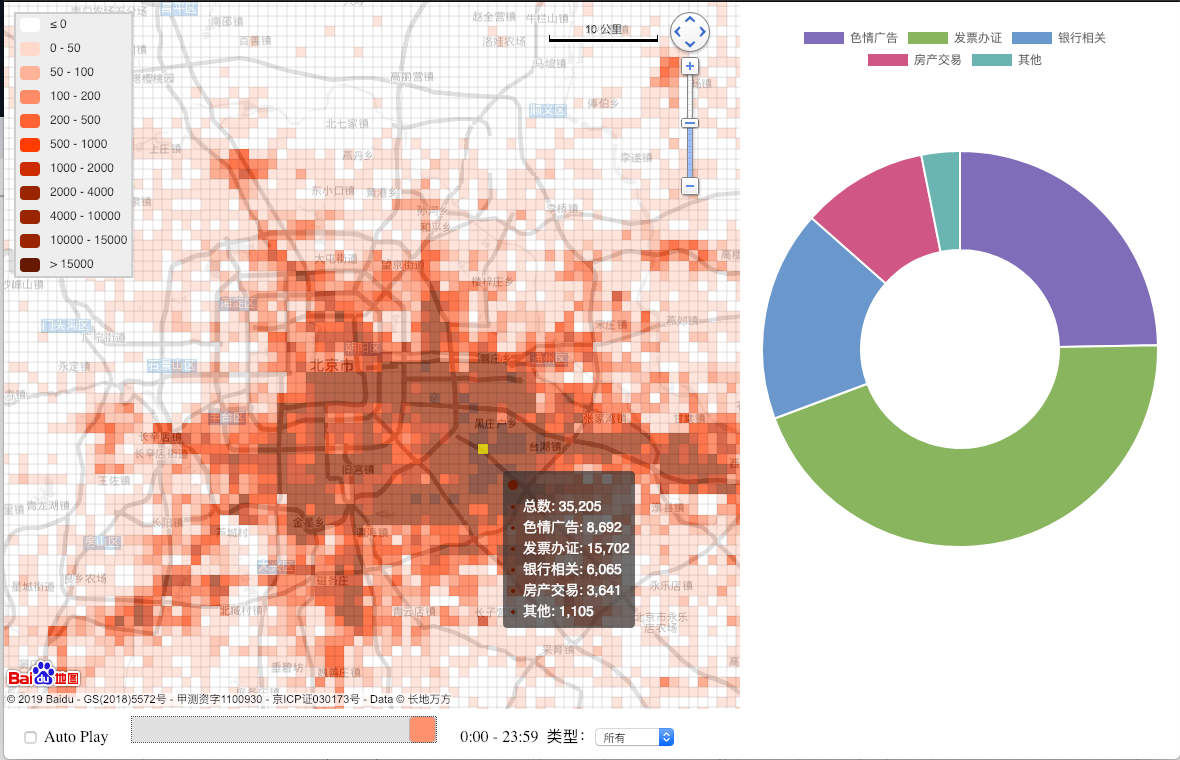
\includegraphics[width=\linewidth]{pic1.png}
		\caption{不同地区垃圾短信数量}
\end{figure}
\end{flushleft}
	

而为了能够了解垃圾短信在时间上的分布规律,我们提供了按照小时查看我们的可视化结果的功能。用户可以通过选择其要查看的具体小时,或者
使用自动播放功能来对不同时段垃圾短信的发送情况有一个具体的了解。

\begin{flushleft}
	\begin{figure}[H]
		\centering
			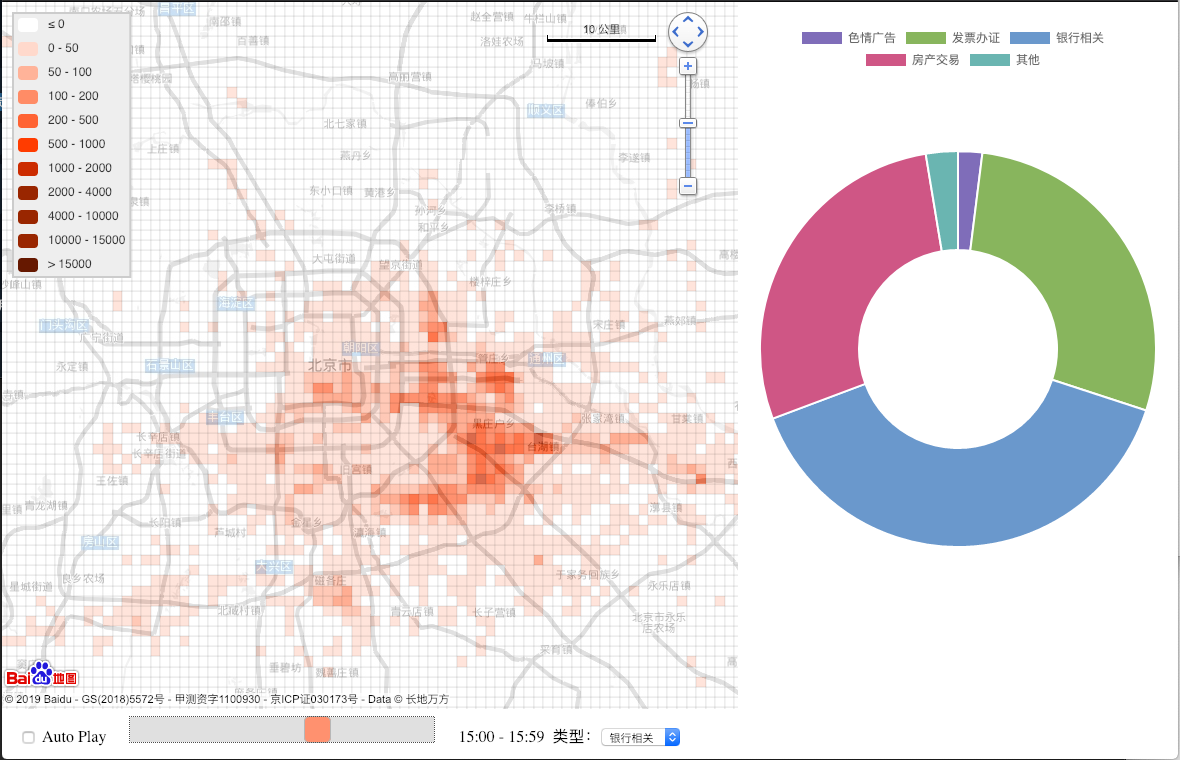
\includegraphics[width=\linewidth]{pic3.png}
			\caption{按类型和时间查看}
	\end{figure}
\end{flushleft}

为了打击垃圾短信,我们需要有针对性地根据不同的垃圾短信类型选择不同的对策。我们同样是通过可视化的方法,根据每个地区主要的垃圾短信的
类型为每个小方格标记上不同的颜色,从而得以让我们对不同地区的主要垃圾短信类型有一个更为直观的理解,从而得以针对不同地区制定
更为有效的治理策略。此外,用户还可以通过选择不同时间查看或是自动播放的功能,来查看不同时段不同种类的垃圾短信的分布规律。

\begin{flushleft}
	\begin{figure}[H]
		\centering
			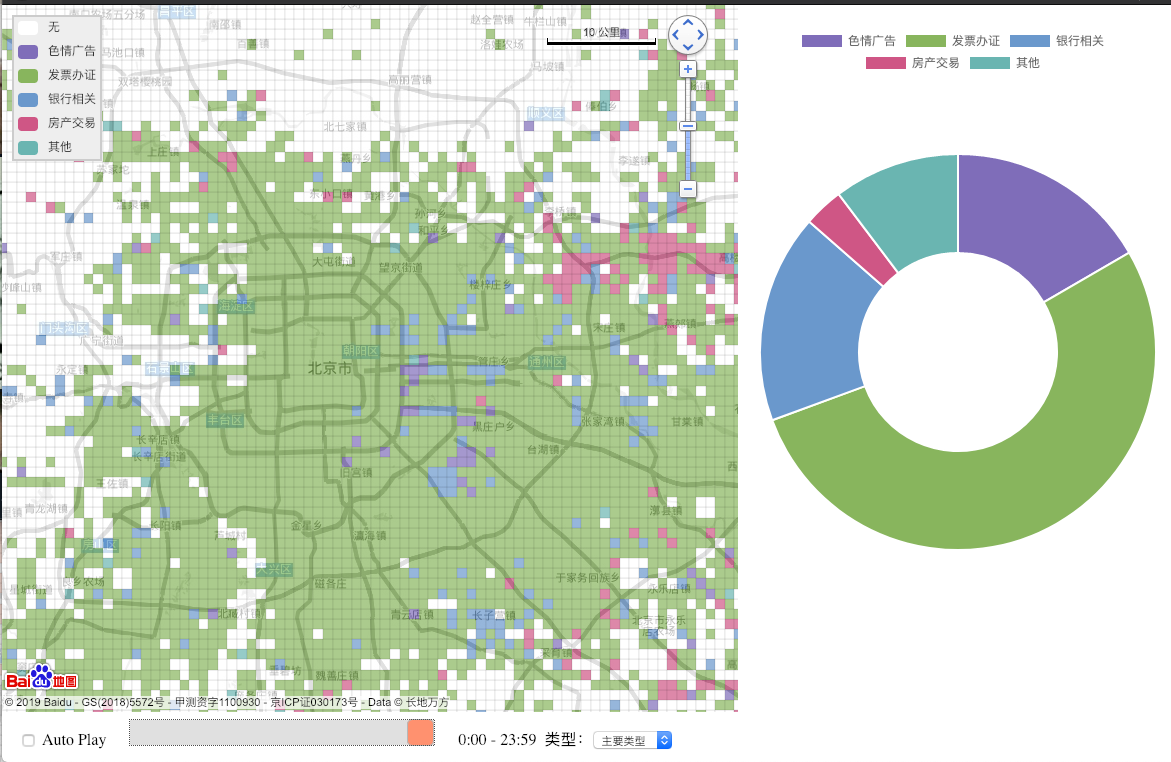
\includegraphics[width=\linewidth]{pic2.png}
			\caption{不同地区主要垃圾短信类型}
	\end{figure}
\end{flushleft}

\section{案例展示}

\begin{itemize}
	\item \textbf{请从宏观时空分析的角度出发,对垃圾短信数据进行可视分析,揭示伪基站的总体时空活动规律。}
	
	首先我们来看看北京伪基站的整体分布情况。
	从上图我们可以看到,在整个北京的范围内,
	大部分地区可以说都是有被伪基站所侵扰的。
	而且从地图上我们可以直观的看出,从整体上来说北京城南地区的伪基站可以说是远多于城北地区的且垃圾短信的
	发送量同样远大于城北地区,因而我们需要重点关注
	城南地区的伪基站。

	\begin{flushleft}
		\begin{figure}[H]
			\centering
				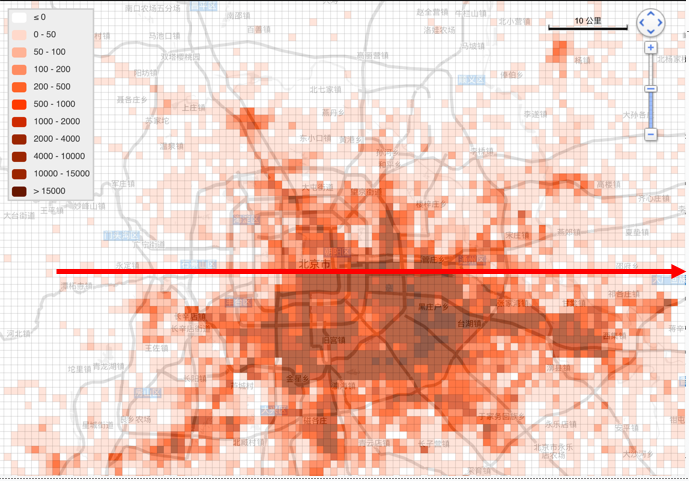
\includegraphics[width=\linewidth]{pic4.png}
				\caption{北京总体垃圾短信分布}
		\end{figure}
	\end{flushleft}

	接下来我们可以放大地图,我们可以发现,在朝阳区的垃圾短信的分布相较于其他地区十分密集,且发送量较大。
	同样我们可以看出,在朝阳地区,在人口密集处的亦庄以及经济不发达地区如黑庄户乡,垃圾短信的数量相较于其他地区同样
	也较多。

	\begin{flushleft}
		\begin{figure}[H]
			\centering
				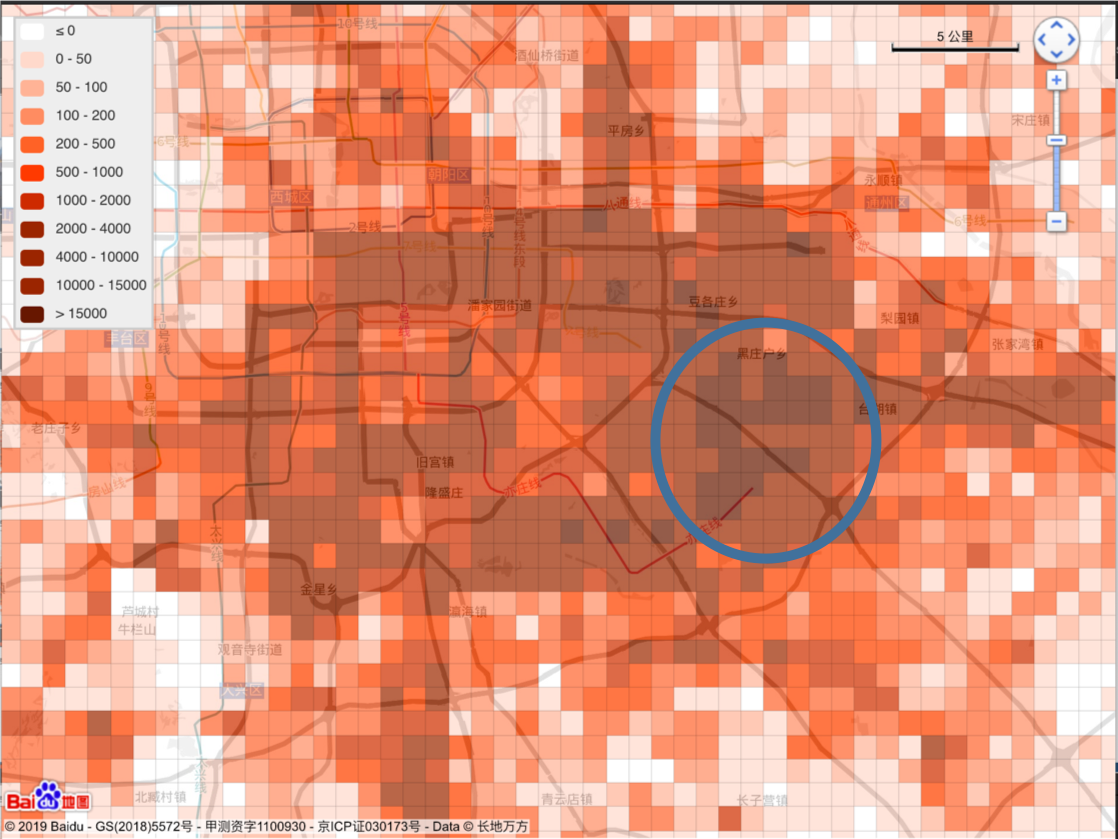
\includegraphics[width=\linewidth]{pic5.png}
				\caption{朝阳地区垃圾短信分布}
		\end{figure}
	\end{flushleft}

	此外,我们还可以发现,在交通沿线之处,垃圾短信的活动也较为猖獗。

	\begin{flushleft}
		\begin{figure}[H]
			\centering
				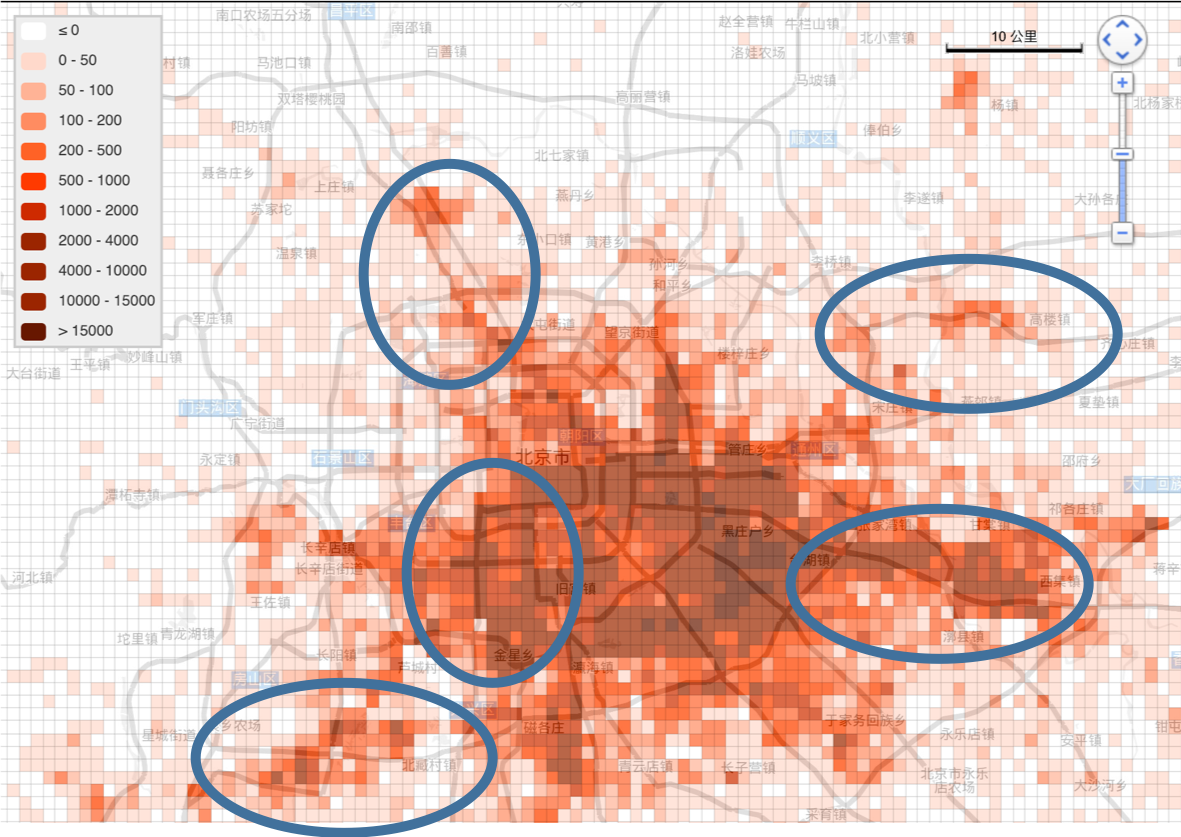
\includegraphics[width=\linewidth]{pic6.png}
				\caption{交通干线垃圾短信分布}
		\end{figure}
	\end{flushleft}

	而接下来,我们从上免的几张对比图中我们可以看出,伪基站的工作可以说是有很大的时间上的规律的。
	从上面几张对比图我们可以看到,在早上7点的时候伪基站的数量开始增多,然后10:00之时达到顶峰,而从18:00之后又开始
	逐步减少,最终在凌晨十分活动基本停止。

	\begin{flushleft}
		\begin{figure}[H]
			\centering
				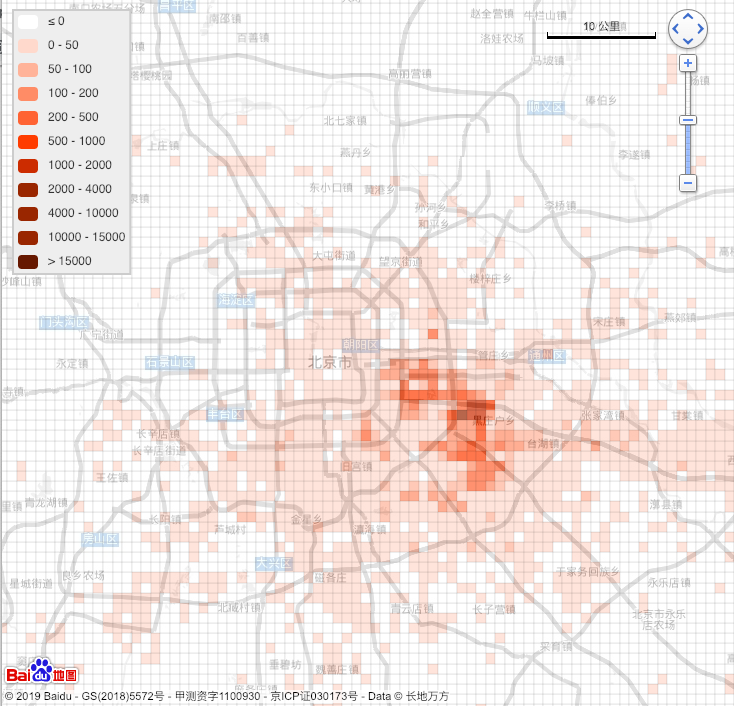
\includegraphics[width=\linewidth]{7.png}
				\caption{7:00 时垃圾短信分布}
		\end{figure}
	\end{flushleft}

	\begin{flushleft}
		\begin{figure}[H]
			\centering
				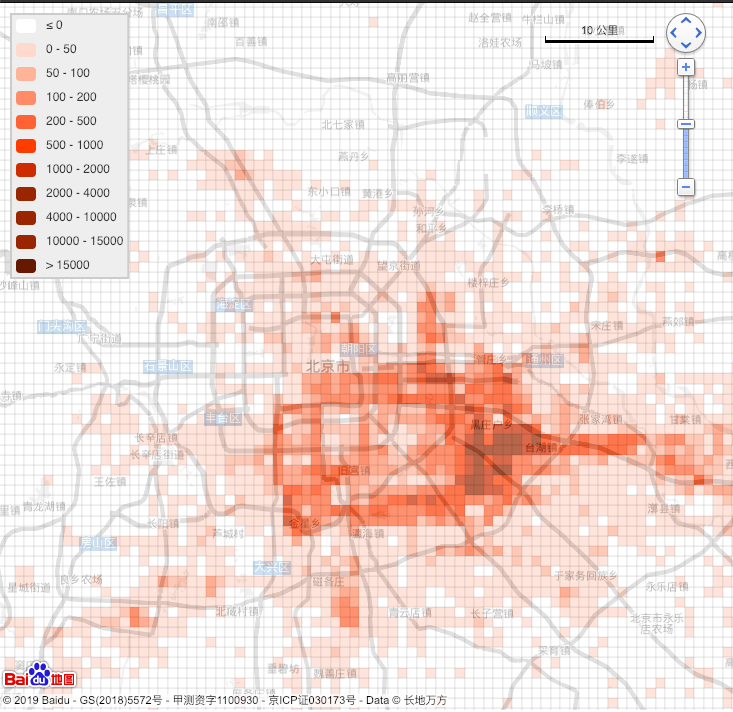
\includegraphics[width=\linewidth]{10.png}
				\caption{10:00 时垃圾短信分布}
		\end{figure}
	\end{flushleft}

	\begin{flushleft}
		\begin{figure}[H]
			\centering
				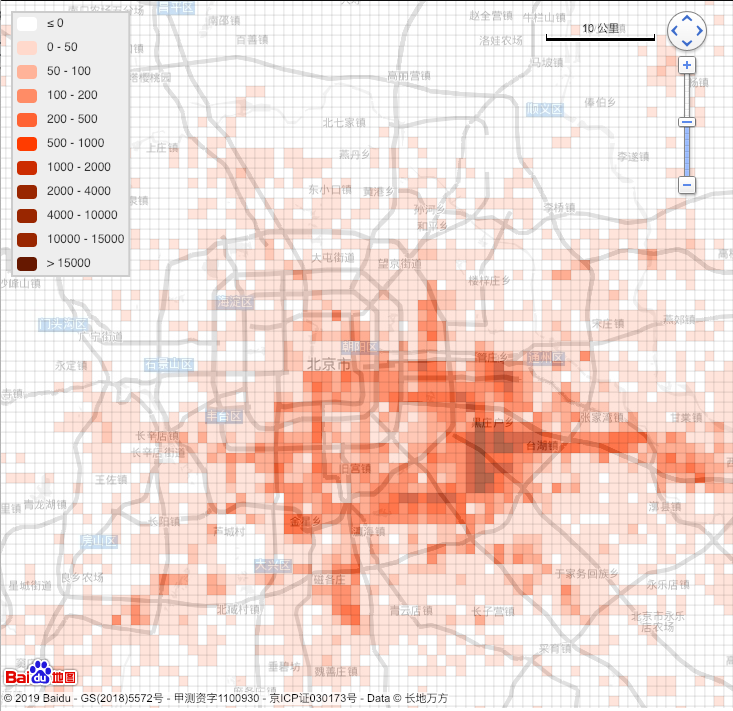
\includegraphics[width=\linewidth]{18.png}
				\caption{18:00 时垃圾短信分布}
		\end{figure}
	\end{flushleft}

	\begin{flushleft}
		\begin{figure}[H]
			\centering
				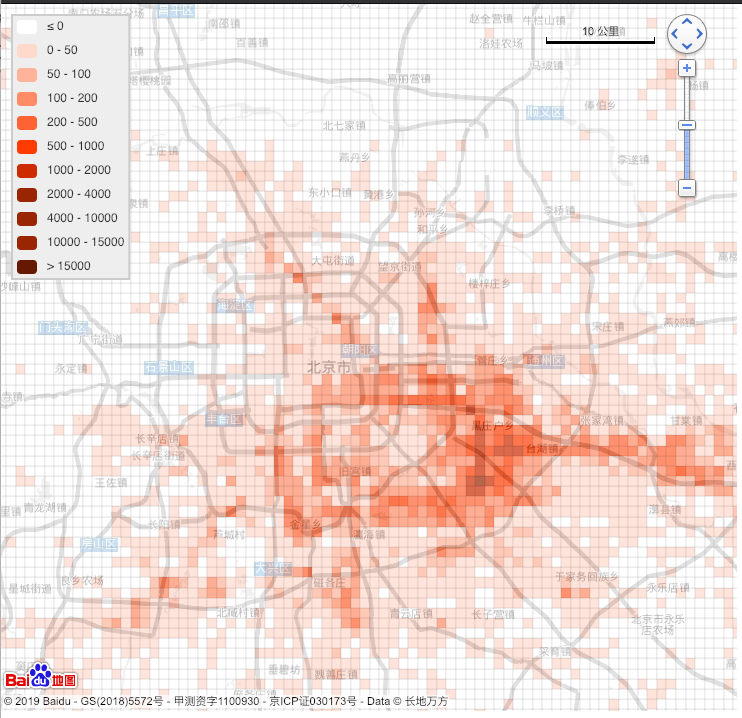
\includegraphics[width=\linewidth]{23.png}
				\caption{23:00 时垃圾短信分布}
		\end{figure}
	\end{flushleft}

	\item \textbf{请尝试在问题1的基础上进一步分析伪基站发送不同类型垃圾短信的时空分布规律。}

	我们在判别垃圾短信的类型之上,我们采用了简单的关键词匹配的方法进行操作。例如,我们可以利用
	银行、信用卡、额度等来关键词来识别银行相关的诈骗短信。而从我们的实验结果上来看,我们简单的关键词匹配可以说是能够
	准确地为超过95\%的垃圾短信进行分类。

	\begin{flushleft}
		\begin{figure}[H]
			\centering
				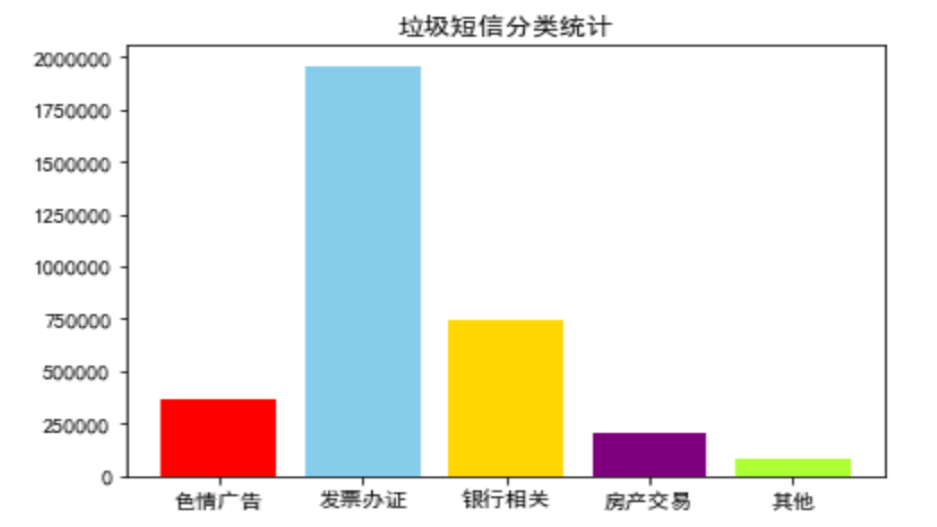
\includegraphics[width=\linewidth]{pic7.png}
				\caption{垃圾短信类型整体统计}
		\end{figure}
	\end{flushleft}

	从上图中我们可以非常直观地看出,若是以种类进行分类的情况下,发票办证类得了垃圾短信的数量可以说是远远超出其他类型的
	垃圾短信的。而第二多的垃圾短信类型则是银行相关类的垃圾短信,其次是色情广告以及房产交易类的垃圾短信。

	\begin{flushleft}
		\begin{figure}[H]
			\centering
				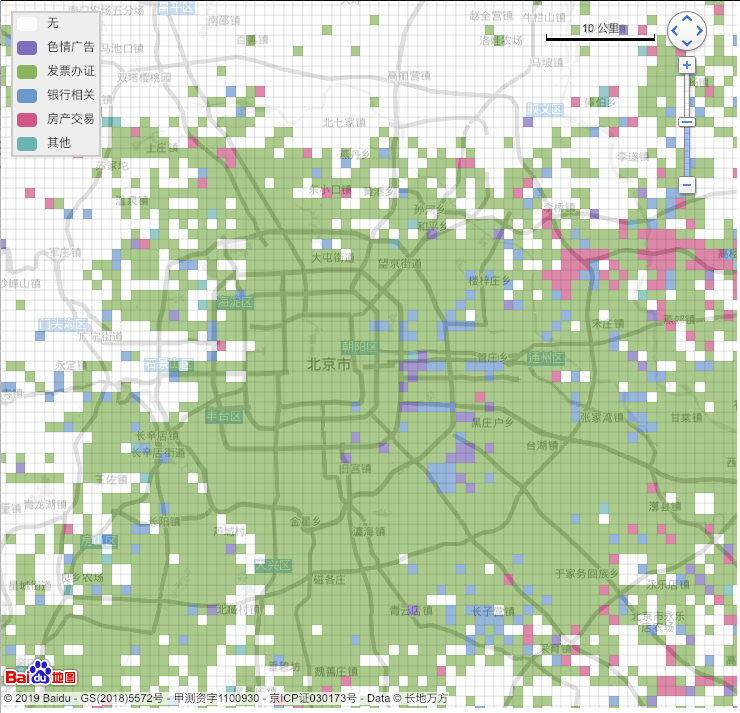
\includegraphics[width=\linewidth]{full.png}
				\caption{地区主体垃圾短信统计}
		\end{figure}
	\end{flushleft}

	接下来我们来看看北京地区各个区域的主要垃圾短信类型。从上图中我们可以看见,浅蓝色的格子可以说是覆盖了绝大多数的
	北京城区,所以从上图中我们可以发现,对于绝大多说的伪基站来说,其发送的最主要的垃圾短信类型还是发票办证相关的信息。
	而从地图的右上角我们也可以清楚地看到,有一片绿色的地区是以房产交易类的垃圾短信为主的。我们通过拉近地图可以发现
	其为燕郊地区,而此地区的房地产近期由于调控而价格有了大幅度的松动,而这一原因也很好地解释了其独特的垃圾短信分布的原因。
	所以我们可以发现,垃圾短信的分布是具有地域特色的。

	接下来我们来分析不同垃圾短信类型的发送规律。我们可以发现,在大部分时段垃圾短信都是以发票办证类为主的,特别是在凌晨时段,但
	0:00-2:00 的时候仍有少量色情服务类的短信。而随着时间的推移,从9:00开始之后银行诈骗类的短信开始增多、出现,而在15:00
	之后又开始逐步消失,而这一分布规律恰好与银行的工作时间相重合。
	除此之外,我们还可以发现,市中心以及城北大多数情况均以发票办证类为主。而至于色情服务类的垃圾短信,我们可以发现
	其大约于夜晚18:00之后开始大量出现,且在此一时段其发送量大大超过了其他类型的垃圾短信。随后其发送量逐渐减少,并在灵成基本消失。
	此外,其发送的地方同样集中于人口较多之处。

	\begin{flushleft}
		\begin{figure}[H]
			\centering
				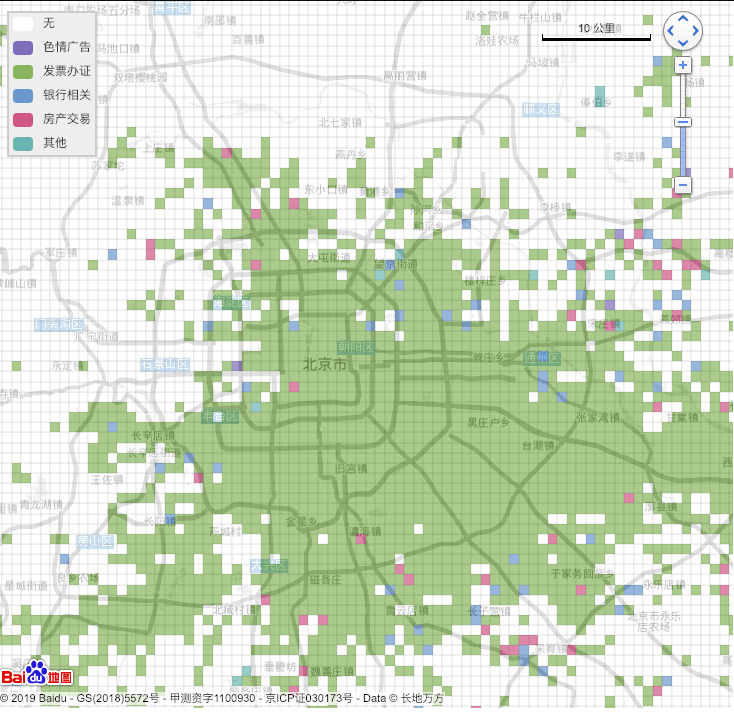
\includegraphics[width=\linewidth]{2-7.png}
				\caption{7:00 时垃圾短信分布}
		\end{figure}
	\end{flushleft}

	\begin{flushleft}
		\begin{figure}[H]
			\centering
				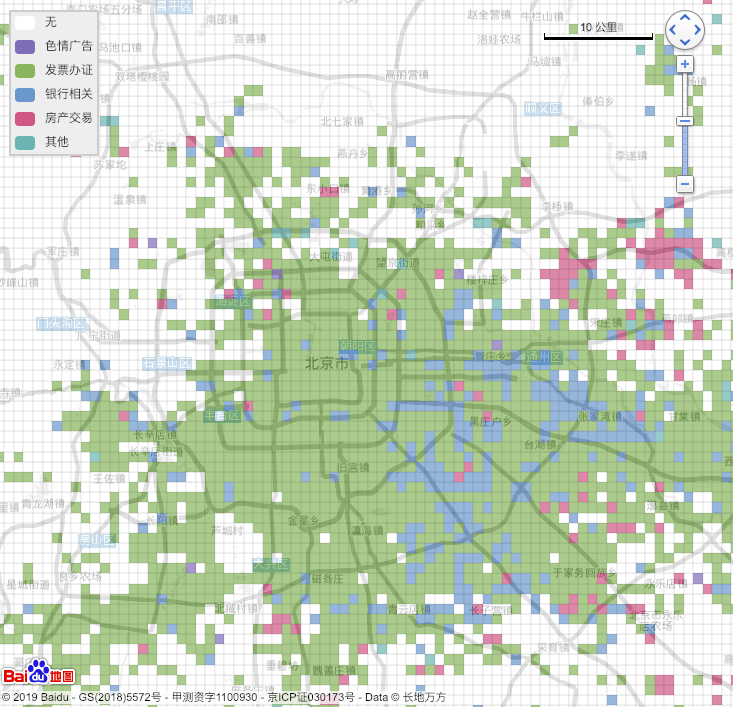
\includegraphics[width=\linewidth]{2-11.png}
				\caption{11:00 时垃圾短信分布}
		\end{figure}
	\end{flushleft}

	\begin{flushleft}
		\begin{figure}[H]
			\centering
				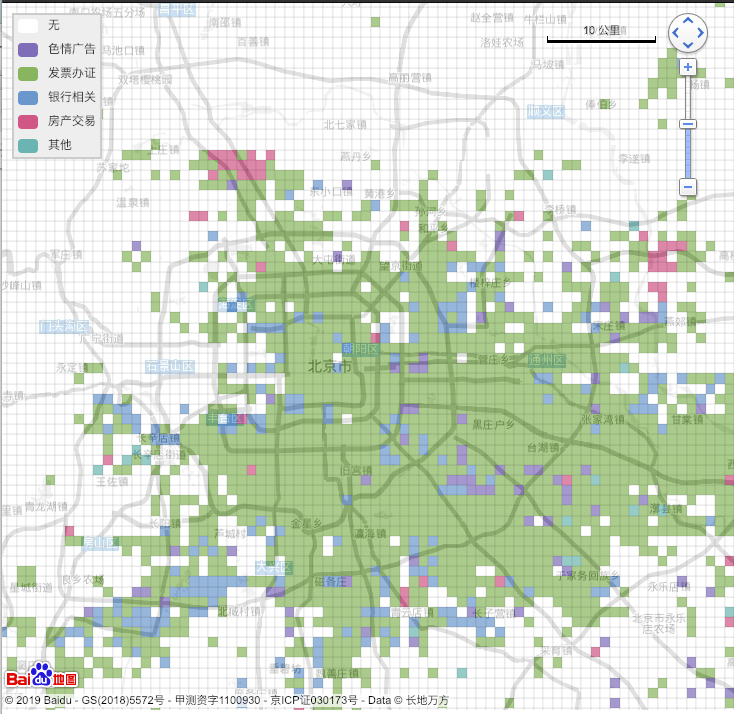
\includegraphics[width=\linewidth]{2-18.png}
				\caption{18:00 时垃圾短信分布}
		\end{figure}
	\end{flushleft}

	\begin{flushleft}
		\begin{figure}[H]
			\centering
				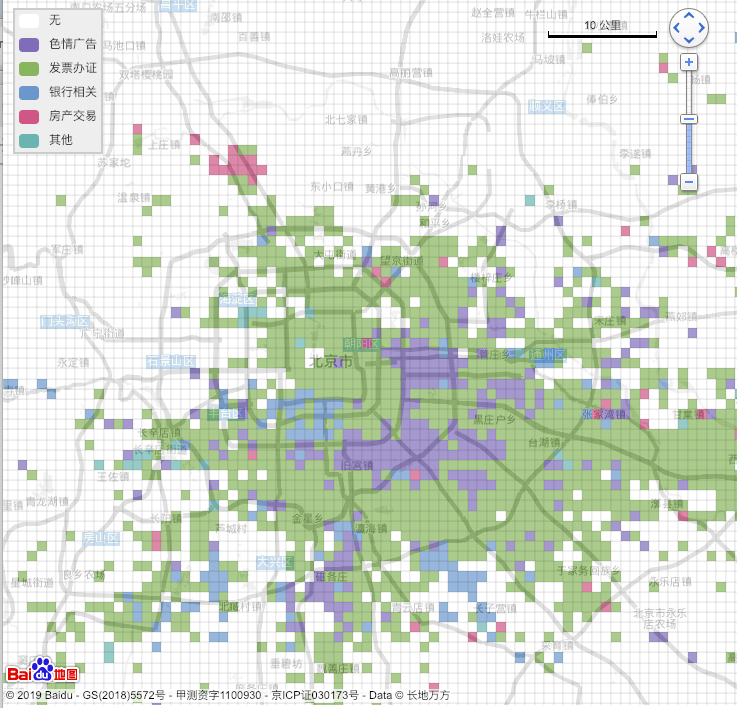
\includegraphics[width=\linewidth]{2-20.png}
				\caption{20:00 时垃圾短信分布}
		\end{figure}
	\end{flushleft}

	

	\item \textbf{请结合以上两题中得到的伪基站行为模式,向执法人员提出打击整治伪基站的有效建议和方案,并结合数据分析结果进行说明。}
	
	\begin{itemize}
		\item 首先,执法人员可以根据伪基站的地理分布特征,对伪基站较为严重的地带如朝阳区进行重点整治和打击。例如,其可以根据
		我们可视化结果中首先对颜色较深的部分进行重点排查,对进出此地区的人员以及车辆加大检查力度,以加大对
		伪基站设备以及伪基站操作人员的查住。

		除此之外,由于伪基站多分布在主要交通线路如地铁、环路等人流密集处,执法人员同样可以利用此特点,在交通干道
		沿线加强检查。

		\item 除此之外,执法人员同样可以利用伪基站的时间分布规律,来对其进行打击。比如从我们的可视化分析结果可以看出,
		伪基站多半从七点多开始工作。因而执法人员可以利用这一规律而了解到伪基站操作人员的作息规律,
		从而得以在对应时段加强巡逻力度,从而加大抓获操作伪基站人员的可能性。

		\item 再次,执法人员也可以根据不同时段伪基站发送的主要短信类别,来针对不同的垃圾短信类型制定不同的打击策略。
		例如,从我们的可视化结果中我们可以清楚地发现,在某些地区色情服务业可以说是十分发达的,因而执法人员可以考虑联合
		其他的执法部门来对此一区域加大扫黄打非的力度,进而达到减少色情服务业从业人员数量的效果,从而得以间接地减少色情服务类型
		垃圾短信的数量。
		
		\item 另外,我们也不应该忽略对群众进行教育的重要性。我们可以利用可视化的结果,在伪基站的高发地段加强对群众的教育
		工作,让老百姓对于伪基站有更多的认识,从而得以让普通群众在遭受例如伪基站发送的银行诈骗类短信之时,有更低的可能性会
		上当受骗,受到实际上的精神损失以及经济损失。

	\end{itemize}

\end{itemize}


\end{document}
